 \documentclass{report}
 
\usepackage[utf8]{inputenc} 
\usepackage[T1]{fontenc}      
\usepackage[top=2.0cm, bottom=3cm, left=3.0cm, right=3.0cm]{geometry}
\usepackage{graphicx}
\usepackage{wrapfig}
\usepackage{amsmath,esint }
\usepackage{amssymb}
\graphicspath{{figures/}{../figures}}

\newcommand*\dif{\mathop{}\!\mathrm{d}}
\newcommand*\diver{\mathop{}\!\mathrm{div}}
\newcommand*\grad{\mathop{}\!\mathrm{grad}}

\begin{document}

\section*{Force exercée sur un barrage}

\begin{itemize}

	\item[$\diamond$] Il s'agit de la démonstration classique de l'équation de statique des fluides. Le bilan des forces (pression et gravité) sur un volume élémentaire $\dif V=\dif x \dif y \dif z$ d'air situé au point $M=(x,y,z)$ s'écrit
	\begin{align*}
		-P(x,y,z+ \dif z)\dif x\dif y\vec{e}_z+P(x,y,z)\dif x\dif y\vec{e}_z+\rho\vec{g}=\vec{0}
	\end{align*}
	On omis les variations de pression selon $x$ et selon $y$ mais qui sont traitées de la même manière qu'en $z$. On trouve alors rapidement l'expression $\vec{\grad}(P) + \rho\vec{g}=\vec{0}$ avec le développement de Taylor de $P(z+dz)$.
	
	\item[$\diamond$] En utilisant la relation précédente : 
	
	\begin{align*}
		p(z) = p_0+\rho g (H-z)
	\end{align*}
		
		\item[$\diamond$] Il faut faire un bilan des forces, en "zoomant" sur la paroi du barrage en un point $(x,z)$ de la surface. La force élémentaire créée par la pression est $d\vec{F}=p(x)dS\vec{n}$, où $\vec{n}$ est la normale à la surface : $\vec{n}=\sin\alpha\vec{e}_x-\cos\alpha\vec{e}_z$, en notant $\alpha$ l'angle la pente du barrage en ce point, cad $\tan\alpha=dz/dx$.
		
		Pour la force horizontale, selon $\vec{e_x}$ :
		
	\begin{align*}
		dF_x = p(z)\sqrt{dx^2+dz^2}L\sin\alpha=p(z)Ldz
	\end{align*}
	car $dS = Ldl=\sqrt{dx^2+dz^2}L$ et $\sin\alpha=dz/dl$. On a donc :
	\begin{align*}
		F_x = \int_0^H p(z)Ldz=\left[ p_0+\frac{\rho g H}{2}\right] LH
	\end{align*}
	
		Pour la force verticale, selon $\vec{e_z}$ :
		
	\begin{align*}
		dF_z= p(z)\sqrt{dx^2+dz^2}L\cos\alpha = -p(z)Ldx
	\end{align*}
	car $\cos\alpha=dx/dl$. En posant $x_0$ tel que $H=kx_0^2$, on a donc :
	\begin{align*}
		F_z = \int_0^{x_0} p(z)Ldz=L\int_0^{x_0} (p_0+\rho g (H-kx^2)dz=-Lx_0p_0-\frac{2}{3}L\rho g x_0H
	\end{align*}

\end{itemize}

\section*{Structure de l'atmosphère}

\begin{itemize}

	\item[$\vartriangle$] Il s'agit de la démonstration classique de l'équation de statique des fluides. Le bilan des forces (pression et gravité) sur un volume élémentaire $\dif V=\dif x \dif y \dif z$ d'air situé au point $M=(x,y,z)$ s'écrit
	\begin{align*}
		-P(x,y,z+ \dif z)\dif x\dif y\vec{e}_z+P(x,y,z)\dif x\dif y\vec{e}_z+\rho\vec{g}=\vec{0}
	\end{align*}
	On omis les variations de pression selon $x$ et selon $y$ mais qui sont traitées de la même manière qu'en $z$. On trouve alors rapidement l'expression $\vec{\grad}(P) + \rho\vec{g}=\vec{0}$ avec le développement de Taylor de $P(z+dz)$.
	
	\item[$\vartriangle$] Dans l'hypothèse d'une transformation adiabatique réversible, un volume $V$ d'air changeant d'altitude suit la loi de Laplace $PV^\gamma=cste$. Comme la densité $\rho$ du gaz contenu dans ce volume $V$ est inversement proportionnelle à celui-ci, on a :
	\begin{align*}
		\rho = cste\times P^{1/\gamma}
	\end{align*}
	Pour déterminer la constante, on utilise la loi des gaz parfait à l'altitude $z_0$ : $P_0V=nRT_0$, ce qui donne $\rho_0=\frac{MP_0}{RT_0}$. On a donc :
	\begin{align*}
		\rho = \rho_0\left(\frac{P}{P_0} \right) ^{1/\gamma}=\frac{MP_0}{RT_0}\left(\frac{P}{P_0} \right) ^{1/\gamma}
	\end{align*}
	
	\item[$\vartriangle$] Avec l'équation de statique des fluide, on a donc :
	\begin{align*}
		\frac{\dif P}{\dif z}=-\rho g = -\frac{Mg}{RT_0}P_0\left(\frac{P}{P_0} \right) ^{1/\gamma}
	\end{align*}
	On introduit le paramètre $H=\frac{RT_0}{Mg}$ homogène à une altitude et la variable de pression réduite $p=P/P_0$. L'équation différentielle devient alors :
	\begin{align*}
		\frac{\dif p}{\dif z}=-\frac{1}{H}p^{1/\gamma}
	\end{align*}	
	La solution est alors :
	
\noindent\fbox{\parbox{\linewidth\fboxrule\fboxsep}{
	\begin{align*}
		p(z)=\left(1-\frac{\gamma-1}{\gamma}\frac{z}{H} \right)^{\frac{\gamma}{\gamma-1}}
	\end{align*}
	}}
	
	La densité se trouve grâce à la relation explicitée à la question précédente :
	
\noindent\fbox{\parbox{\linewidth\fboxrule\fboxsep}{
	\begin{align*}
		\rho(z)=\frac{P_0}{Hg}\left(1-\frac{\gamma-1}{\gamma}\frac{z}{H} \right)^{\frac{1}{\gamma-1}}
	\end{align*}
	}}	
	
	La température se trouve grâce à la relaiton de Laplace, $T^\gamma P^{1-\gamma}=cste$. On a alors $T=T_0\left( \frac{P}{P_0}\right)^\frac{\gamma-1}{\gamma}=T_0p^\frac{\gamma-1}{\gamma}$, donc :
	 
	 	
\noindent\fbox{\parbox{\linewidth\fboxrule\fboxsep}{
	\begin{align*}
		T(z)=T_0\left(1-\frac{\gamma-1}{\gamma}\frac{z}{H} \right)
	\end{align*}
	}}

Les fonctions $P$, $\rho$ et $T$ ne sont définies si et seulement si $1-\frac{1-\gamma}{\gamma}\frac{z}{H}>0$, cad si $z<\frac{\gamma}{\gamma-1}H\simeq 29.75$km. Il n'y a plus du tout de gaz au-delà !

	\item[$\vartriangle$]  La température décroit linéairement avec l'altitude, c'est un résultat que l'on retrouve expérimentalement : plus on monte, plus il fait froid ! Plus précisément, elle diminue de $T_0\frac{\gamma}{1-\gamma}\frac{1}{H}\simeq9.77\cdot10^{-3}$ $^{\circ}$C pour une élévation de 1m, soit une chute de 9.77$^{\circ}$C pour 1000m. 
	
	Au sommet de l'Everest, la pression est de seulement 1/3 celle au niveau de la mer, et la densité seulement la moitié.
	
\begin{figure}[!h]
	\centering
	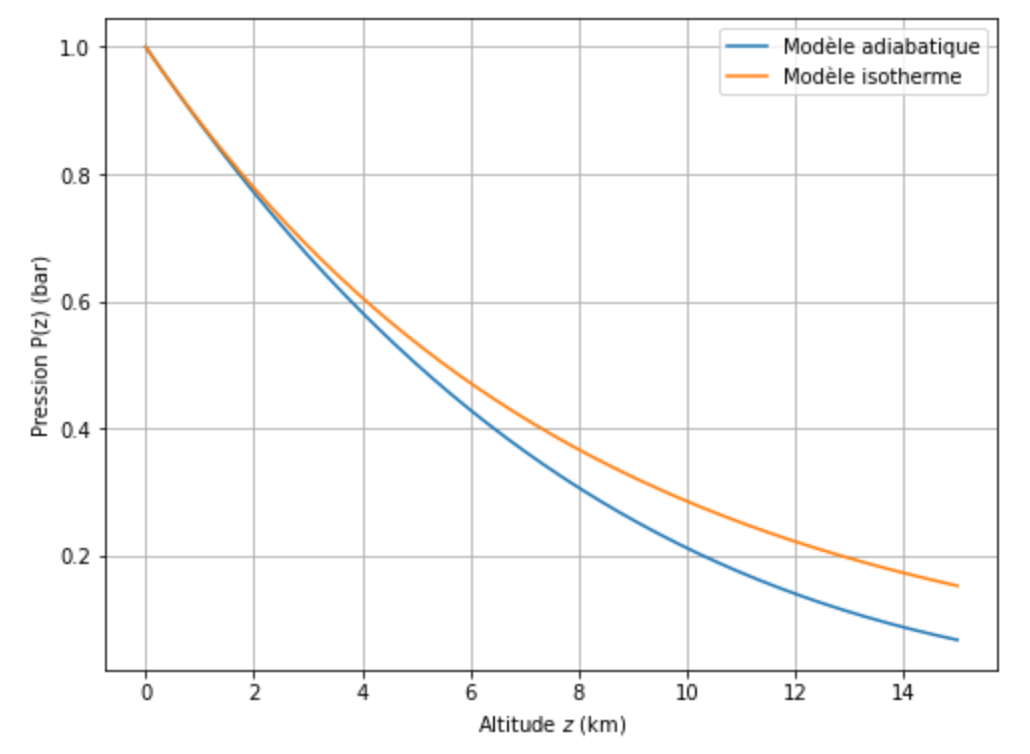
\includegraphics[width=0.5\linewidth]{exo_atmo1.png}
\end{figure}
\begin{figure}[!h]
	\centering
	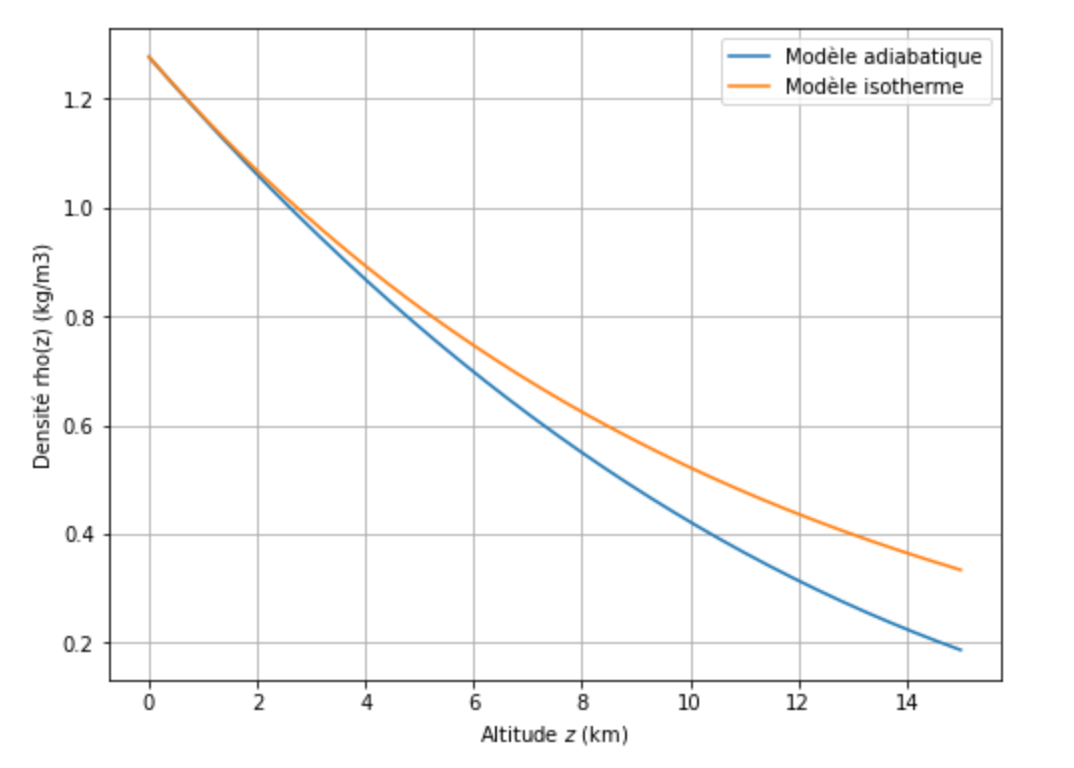
\includegraphics[width=0.5\linewidth]{exo_atmo2.png}
\end{figure}
\begin{figure}[!h]
	\centering
	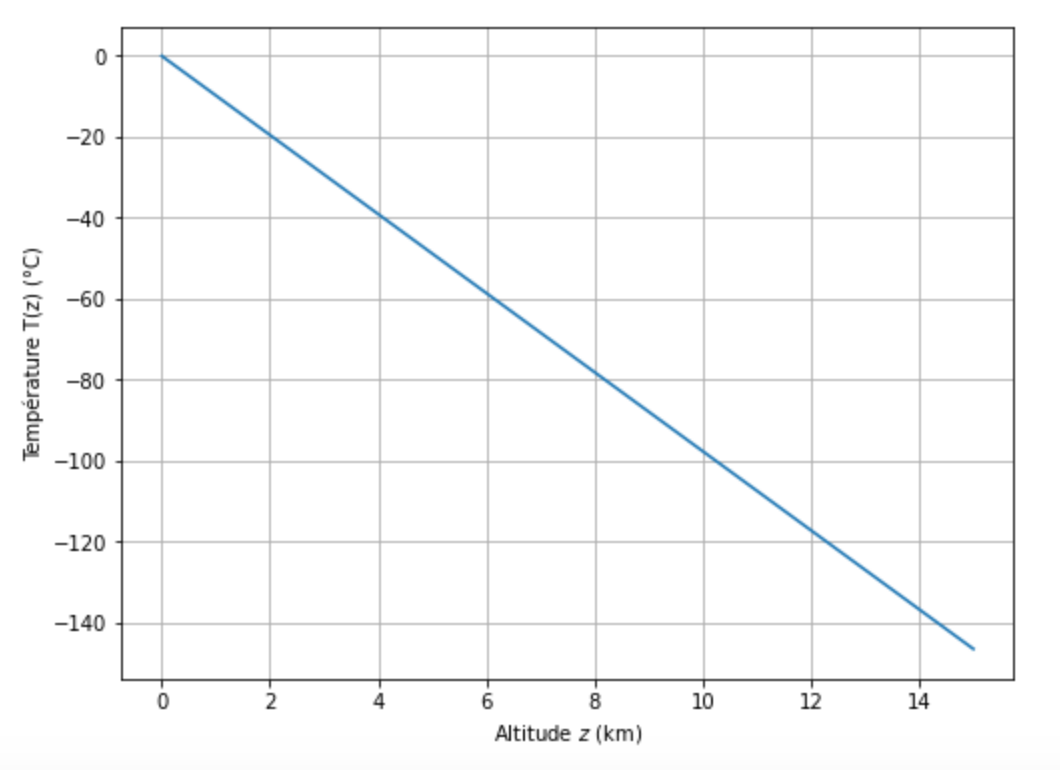
\includegraphics[width=0.5\linewidth]{exo_atmo3.png}
\end{figure}

	\item[$\vartriangle$] L'atmosphère réelle permet des échanges thermiques même faibles. Le gradient de température est un peu plus faible, et coefficient thermodynamique $\gamma_{eff}$ est plus faible, correspondant à une situation où l'on est pas parfaitement adaibatique. Pour le retrouver, on utilise le gradient de température :
	\begin{align*}
		\frac{\dif T}{\dif z}=-T_0\frac{\gamma-1}{\gamma H}=-Mg\frac{\gamma-1}{\gamma R}
	\end{align*}
Pour $\frac{\dif T}{\dif z}=-7.7\cdot10^{-3}$K.m$^{-1}$, on trouve $\gamma_{eff}=1,26$.

	\item[$\vartriangle$] Le modèle d'atmosphère isotherme correspond au cas où $\gamma_{eff}=1$. En effet, dans ce cas là on retrouve la loi des gaz parfait $PV=cste=nRT$, on voit aussi que l'atmosphère a un graident de température nulle et une extension infinie : $z<\frac{\gamma}{\gamma-1}H\longrightarrow\infty$. D'autre part, les fonctions pécédentes convergent vers la décroissance exponentielles de l'atmosphère isotherme :
	\begin{align*}
		P(z)&=P_0\left(1-\frac{\gamma-1}{\gamma}\frac{z}{H} \right)^{\frac{\gamma}{\gamma-1}}\\
		&=P_0\exp\left(\frac{\gamma}{\gamma-1}\ln\left(1-\frac{\gamma-1}{\gamma}\frac{z}{H} \right)\right) \\
		&\xrightarrow[\gamma\to1]{} P_0\exp\left(-\frac{z}{H} \right) 
	\end{align*}

\end{itemize}

\section*{Exercice 1}

\begin{itemize}
	\item[•] Avec les hypothèses : $\eta\Delta \vec{v} = \vec{grad}P$. On néglige la variation due à la gravité à l'échelle de la taille de la sphère.  
	\item[•] On cherche à connaitre le champ de pression pour connaitre la résultante des forces. 
	Liquide incompressible donc $div \vec{v}=0$ et donc $\vec{rot}(\vec{rot}(\vec{v}))=\vec{grad} (div \vec{v})-\Delta \vec{v}=-\Delta \vec{v}$, donc le gradient de pression vaut l'opposé l'expression de la vitesse donné plus haut.
	
	En choisissant une projection sur $\vec{e_r}$ ou $\vec{e_\theta}$ (ce qui revient au même) :
	\begin{align*}
		\frac{\partial P}{\partial r} = 3\eta\frac{Rv_\infty}{r^3}\cos\theta 
	\end{align*}
	
	\begin{align*}
		P = -3\eta\frac{Rv_\infty}{2r^2}\cos\theta + P_\infty
	\end{align*}
En notant $P_\infty$ la pression qui est dans le liquide loin de la sphère.

La résultante des forces de pression, selon l'axe $\vec{e_z}$, est $F_{p,z}=-P(M)d\vec{S}\vec{e_z}$. Alors :
\begin{align*}
	F_{p,z} = -\iint P_\infty R^2d\varphi \sin\theta d\theta \cos\theta + \iint 3\eta\frac{Rv_\infty}{2R^2}\cos^2\theta \sin\theta R^2d\theta d\varphi
\end{align*}
\noindent\fbox{\parbox{\linewidth\fboxrule\fboxsep}{
On trouve alors : $F_{p,z}=2\pi\eta v_\infty R$
}}

\item[•] La force de cisaillement correspond à la force de frottement due à la viscosité du fluide. Pour un élément de surface $\vec{dS}$ de la sphère, celle-ci s'écrit :
\begin{align*}
	d\vec{F_c}=\eta dS \frac{\partial v}{\partial r}\vec{e_\theta}
\end{align*}
La projection suivant $\vec{e_z}$ nous donne alors :

\noindent\fbox{\parbox{\linewidth\fboxrule\fboxsep}{
\begin{align*}
	F_{c,z}=\iint \eta \frac{\partial v}{\partial r}R^2\sin\theta d\theta d\varphi \sin\theta=\iint \eta\frac{3}{2}Rv_\infty \sin^3\theta d\theta d\varphi=4\pi\eta Rv_\infty
\end{align*}
}}
L'intégrale sur $\theta$ vaut 4/3.

\item[•] La force de trainée est la somme des deux forces précédentes. On a donc : $F_z = 6\pi\eta Rv_\infty$.
\end{itemize}

\section*{Exercice 2}

\begin{itemize}
	
	\item[$\blacktriangleright$] Les forces s'exerçant sur le fluide sont celles de gravité, de pression et de viscosité. Le bilan des forces s'écrit : 

\begin{align*}
	0=\eta \Delta \vec{v}+\rho\vec{g}-\vec{grad}(P)
\end{align*}
	En projettant sur les axes $x$ et $z$, on obtient :
	
\noindent\fbox{\parbox{\linewidth\fboxrule-2\fboxsep}{
\begin{equation}
\left\lbrace
\begin{array}{ccc}
\vec{e_x}  & : & \eta\frac{\partial^2 v}{\partial z^2}+\rho g \sin\alpha - \frac{\partial P}{\partial x}=0\\
\vec{e_z}  & : &-\rho g \cos\alpha - \frac{\partial P}{\partial z}=0\\
\end{array}\right.
\end{equation}	
}}

	\item[$\blacktriangleright$] Comme l'écoulement est lent, et invariant selon $x$ et $y$ : l'écoulement ne dépend que de $z$. De plus, comme il est incompressible, $div(\vec{v})=0$, donc $v_z=cste=0$, car la vitesse doit être nécessairement nulle en $z=0$. L'écoulement est donc laminaire et est dirigé selon $\vec{e_x}$ (c'est une hypothèse, on suppose qu'il est dans le sens de la descente) : $\vec{v}(x,y,z)=v(z)\vec{e_x}$.
	
	\textit{NB : }avec un tel profil de vitesse, $(\vec{v}\cdot\vec{grad})\vec{v}$ est identiquement nul, mais on peut directement le négliger ce terme avec l'hypothèse de l'énoncé (écoulement lent et très visqueux).

En intégrant selon $\vec{e_z}$ et avec la condition au limite $P(x,z=h)=P_0$, on obtient :
\begin{align*}
	P(x,z)=P_0+\rho g\cos\alpha (h-z)
\end{align*}
En intégrant selon $\vec{e_x}$, avec la condition aux limites $\frac{\partial v}{\partial z}_{z=h}=0$ (il n'y a pas de forces de cisaillement à l'interface air/fluide) devient alors : 
\begin{align*}
	\frac{\partial v}{\partial z}=\frac{\rho g}{\eta}\sin\alpha(h-z)
\end{align*}
En intégrant une nouvelle fois, avec la condition aux limites $v(z=0)=0$ (continuité  de la vitesse avec le support) :

\noindent\fbox{\parbox{\linewidth\fboxrule-2\fboxsep}{
\begin{align*}
	v(z)=\frac{\rho g}{\eta}\sin\alpha z\left( h-\frac{z}{2}\right) 
\end{align*}
}}

Le profil de vitesse est parabolique.

\item[$\blacktriangleright$] Le débit s'écrit, en prenant comme section un carré de largeur $L\gg h$ pour que les hypothèses de l'énoncé soient valables : 
\begin{align*}
	D=\int_{y=0}^{L}dy\int_{z=0}^h dz\cdot v(z)
\end{align*}
En intégrant, on obtient :

\noindent\fbox{\parbox{\linewidth\fboxrule\fboxsep}{
\begin{align*}
	D=\frac{\rho g}{3\eta}\sin\alpha L h^3
\end{align*}
}}

\item[$\blacktriangleright$] La glace a une densité de 900kg.m$^3$. La vitesse proposée est la vitesse maximale de la glace, car c'est celle en surface. On a donc $\eta\simeq7.1\cdot10^{12}$Pa.s.

On obtient donc, sur une année : $V=D\Delta t\simeq4,73\cdot10^6$m$^3$, soit 4250 tonnes chaque année. 

Il faut garder à l'esprit que ce sont des ordre de grandeurs, car nous n'avons pas pris en compte les conditions aux limites sur les bords (en $y$) du canal d'écoulement du glacier, et que la vitesse est elle aussi un ordre de grandeur. 

\item[$\blacktriangleright$] Les conditions aux limites deviennent alors $v(z=0)=v(z=h)=0$, mais on a plus la condition sur la dérivée première de la vitesse. 
La vitesse s'écrit : $v(z)=-\frac{\rho g}{2\eta}\sin\alpha z^2 +a +b$
Avec les conditions aux limites, on trouve $b=0$ et $a=\frac{\rho g}{2\eta}\sin\alpha h$.

\noindent\fbox{\parbox{\linewidth\fboxrule-2\fboxsep}{
\begin{align*}
	v(z)=\frac{\rho g}{2\eta}\sin\alpha z\left( h-z\right) 
\end{align*}
}}

C'est un écoulement de Poiseuille. 

\end{itemize}

\newpage

\section*{Exercice 3}

\begin{itemize}
	\item[1 - ] Dans l'énoncé, le problème est dit invariant en $\theta$ donc la vitesse ne dépend pas de $\theta$. D'autre part l'équation de conservation s'écrit, comme le fluide est incompressible : $div(\vec{v})=0$, cad $\partial u_z/\partial z=0$, cad $u_z$ ne dépend pas de $z$. Finalement, $\vec{u}$ ne dépend que de $r$.
	
	On effectue un bilan de force sur un petit volume en coordonnées cylindrique au point $M(r,\theta,z)$. On projette directement selon $z$ :
	\begin{equation}
		rd\theta drP(z) - rd\theta drP(z+dz) - \eta\tau(r+dr)(r+dr)d\theta dz+ \eta\tau(r)rd\theta dz =0
	\end{equation}
Attention, la définition de $\tau$ implique qu'il est opposé à la variation spatiale de la vitesse. Il y a donc un signe - par rapport aux force classique de cisaillement. 
On obtient la relation voulue :

\noindent\fbox{\parbox{\linewidth\fboxrule-2\fboxsep}{
	\begin{align*}
		\frac{\partial P}{\partial z} + \frac{1}{r}\frac{\partial (r\tau)}{\partial r}=0
	\end{align*}}}

	\item[2 -] On commence à intégrer selon $z$. Étant donné que $u$ ne dépend pas de $z$, $\dot{\gamma}$ non plus, et $\tau$ non plus. Dès lors :
	\begin{align*}
		\int_0^Ldz P(z) = P(L)-P(0)=-\Delta P =-\frac{L}{r}\frac{\partial r\tau}{\partial r}
	\end{align*}
	On obtient donc : $\Delta P =\frac{L}{r}\frac{\partial r\tau}{\partial r}$. On intègre désormais sur $r$, et on trouve la relation demandée. Attention, durant le calcul, on intègre un $r^2$ qui fait aparaître un facteur 1/2. 
	
	\item[3 - ] Pour qu'il y ait écoulement, il faut qu'il existe une valeur de $r$ telle que $\tau>\tau_s$ (car sinon $\dot{\gamma}=0$). La plus grande valeur de $r$ est le rayon $R$, on doit alors nécessairement avoir $R>R_s$ pour espérer voir un écoulement. On a alors $\tau_s = \tau_s R/R_s$.

\noindent\fbox{\parbox{\linewidth\fboxrule-2\fboxsep}{	
	Cela correspond à une pression minimum de $\Delta P_{min}=\frac{2\tau_sL}{R}$.}}
	
	\item[4 - ] Comme $\Delta P > \Delta P_{min}$, on a forcément $R>R_s$. Donc pour $r>R_s$ :
	\begin{align*}
		-\frac{\partial u}{\partial r}=\frac{\tau_s}{\eta}\left( \frac{r}{R_s} - 1\right) 
	\end{align*}
	
\noindent\fbox{\parbox{\linewidth\fboxrule-2\fboxsep}{	
	On trouve donc pour $r>R_s$ :
	\begin{align*}
		u(r) = \frac{\Delta P}{4L\eta}(R+r-2R_s)(R-r)
	\end{align*}
	Pour $r<r_s$, on a $\dot{\gamma}=0$ donc :
	\begin{align*}
	 u(r)=u(R_s)=\frac{\Delta P}{4L\eta}(R-R_s)^2
	 \end{align*}	
}}
	Pour visualiser, l'effet, bouchon, il suffit de tracer la courbe de $u(r)$ en fonction de $r$. 
	
\end{itemize}

\newpage

\section*{Exercice 4}

\begin{itemize}
	\item[1 - ] Il y a deux cas : 
	 
	\begin{itemize}
		\item[$z<0$ : ] Avec l'équation d'incompressibilité $div(\vec{v})=0$, on trouve $\frac{1}{r}\frac{\partial(r v_r}{\partial r}+\frac{\partial v_z}{\partial z} =0$. Comme dans cette partie, les lignes de courants sont parallèle à l'axe $Oz$, la vitesse es tnécessairement selon $e_z$ donc l'équation de conservation devient $\frac{\partial v_z}{\partial z} =0$, don c$v_z=cste=v_0$. Finalement,
		\begin{align*}
			\vec{v}=v_0\vec{e_z}
		\end{align*}
		
		\item[$z>0$ : ] 	La conservation du débit impose que pour toute section du tube, on ait $\iint d\vec{S}\vec{v}= \pi r^2v_z(r,z)=cste$, car $v$ ne dépend pas de $r$. En l'occurrence, pour $z=0$, on a $\pi r^2v_z(r,z)=\pi a^2v_0$. On a donc : 
\begin{align*}
	v_z(r,z)=\frac{a^2}{\left(a+\frac{z^2}{b} \right)^2 }v_0
\end{align*}	

Les lignes de courant sont définies par $\vec{v}\wedge d\vec{l}$. Comme $d\vec{l}=dr\vec{e_r}+dz\vec{e_z}$, donc on a :
\begin{align*}
	v_rdz-v_zdr=0\Longrightarrow \frac{v_r}{v_z}=\frac{\partial r}{\partial z}
\end{align*}
La quantité $\frac{\partial r}{\partial z}$ vaut $2\lambda z/b$. Pour s'affranchir du $\lambda$, il faut l'exprimer en fonction de $r$. En effet, $\lambda$ n'est qu'un paramètre descriptif d'une ligne de champ, qui sera exprimée en fonction de $r$ et $z$ : $\lambda=r/(a+\frac{z^2}{b})$. On a donc :
\begin{align*}
	\frac{\partial r}{\partial z}=\frac{2rz}{ab\left( a+\frac{z^2}{b}\right) }
\end{align*}

\noindent\fbox{\parbox{\linewidth\fboxrule\fboxsep}{	
	On trouve alors :
	\begin{align*}
		\vec{v}=\frac{a^2}{\left(a+\frac{z^2}{b} \right)^2 }v_0\vec{e_z}+\frac{2arz}{b\left( a+\frac{z^2}{b}\right)^3 }v_0\vec{e_r}
	\end{align*}}}
	
	On peut vérifier que l'écoulement est bien incompressible. 
	\end{itemize}

\item[2 - ] Les lignes de courant s'écartent lors du passage dans la zone parabolique, l'élément de fluide se déforme de sorte à être plus fin pour respecter la conservation de la masse. 

\item[3 - ] \begin{align*}
\vec{\Omega}=\vec{rot}(\vec{v})=\left(\frac{\partial v_r}{\partial z}-\frac{\partial v_z}{\partial r} \right)\vec{e_\theta}=\frac{1-5z^2/ab}{\left( 1+z^2/ab\right)^4}\frac{2rv_0}{ab}\vec{e_\theta}\neq 0
\end{align*}

\end{itemize}

\subsubsection*{Écoulement entre deux plaques}

On peut raisonner en superposant les deux champs de vitesse comme en électromagnétisme. 

Il faut séparer le $\ln$ en deux parties pour distinguer les deux vecteurs directeurs correspondant à l'écoulement. On introduit alors $r_0$ une longueur intermédiaire.
\begin{align*}
	\vec{grad}(\phi)=av_0\left(\vec{grad}\ln\frac{r_1}{r_0}-\vec{grad}\ln\frac{r_2}{r_0} \right) 
\end{align*}
On trouve :
\begin{align*}
\vec{v}=av_0\left(\frac{\vec{e_{r_A}}}{r_A}-\frac{\vec{e_{r_B}}}{r_B} \right) 
\end{align*}

Le champs de vitesse créé par la source en A, à une distance $r_A$ de cette source peut s'écrire sous la forme :
\begin{align*}
	\vec{v_A} = v_A(r_A,z)\vec{e_{r_A}}
\end{align*} 
En effet, par invariance, $\vec{v_A}$ ne peut dépendre de $\theta$. D'autre part, comme l'écoulement est lent, il ne pourra être dirigé que selon $\vec{e_{r_A}}$.

Avec la conservation du débit, on a :
\begin{align*}
	D_e = 2\pi r_A\int_{-e/2}^{e/2}dz v(r_A,z)
\end{align*}
En notant $v_{moy}=\frac{1}{e}\int_{-e/2}^{e/2}dz v(r,z)$, qui correspond à la vitesse moyenne entre les deux plaques, on obtient :
\begin{align*}
	\vec{v_{moy}}(r_A) = \frac{D_e}{2\pi r e}\vec{e_{r_A}}
\end{align*}
La vitesse décroit en $1/r_A$. S'il n'ya pas de viscosité, on a bien $v_{moy}=v$.

Même chose pour la source en B :
\begin{align*}
	\vec{v_{moy}}(r_B) = -\frac{D_e}{2\pi r e}\vec{e_{r_B}}
\end{align*}

Au final : 
\begin{align*}
	\vec{v_{moy}} = \frac{D_e}{2\pi e}\left( \frac{1}{r_A}\vec{e_{r_A}} - \frac{1}{r_B}\vec{e_{r_B}}\right) 
\end{align*}

Les champs de vitesses sont à divergence nulle donc incompressibles.

\newpage

\section*{Boîte automatique}

\begin{itemize}
		
	\item[$\bigstar$] Question piège : on a pas la vitesse de rotation. Pour un moteur de voiture, on a typiquement $\Omega=1000$tr/min$\simeq105$rad/s, soit une vitesse typique $U=R_2\Omega\simeq31$m/s. On trouve $Re=\rho UL/\eta\simeq 67$, soit un écoulement laminaire.
	
	\item[$\bigstar$] Comme l'écoulement est incompressible, on a $\mathbf{div}(\vec{v})=0$. Avec les hypothèses de l'énoncé, on trouve donc que $v_r=\frac{cste}{r}$. Comme $v_r(R_1)=0$ par conservation du débit, $\forall r, v_r=0$.
	
	\item[$\bigstar$] Le plus simple est de faire un bilan des moments selon $\vec{e_z}$ à un élément de fluide (en coordonnées cylindriques) qui est un anneau (ou tore) compris entre $r$ et $r+dr$, d'épaisseur $dz$. Les forces visqueuses s'appliquent orthoradialement alors sur les surfaces internes et externe. 

Comme on est en régime stationnaire, le moment total exercé doit être nul de sorte que : 
\begin{align*}
	2\pi r dz \sigma_\theta(r)\times r - 2\pi (r+dr) dz \sigma_\theta(r+dr)\times (r+dr) = 0
\end{align*}
cad : $r^2 \sigma_\theta(r) - (r+dr)^2 \sigma_\theta(r+dr) = 0$. On en déduit que $\frac{\partial}{\partial r}r^2\sigma_\theta=0$.

D'autre part, $\sigma_\theta=\eta\left(\frac{\partial v_\theta}{\partial r}-\frac{v_\theta}{r}\right) =\eta r \frac{\partial}{\partial r}\frac{v_\theta}{r} $. On trouve le résultant voulu :

\noindent\fbox{\parbox{\linewidth\fboxrule-2\fboxsep}{	
	\begin{align*}
		\frac{\partial}{\partial r}\left(r^3 \frac{\partial}{\partial r}\frac{v_\theta}{r} \right) =0
	\end{align*}}}
	
	\item[$\bigstar$] On intègre la relaiton précédente et on trouve :
	\begin{align*}
		v_\theta = \frac{A}{r} + Br
	\end{align*}
	Les conditions aux limites sont : $v_\theta(r=R_{1,2})=R_{1,2}\Omega_{1,2}$. On obtient alors : 
	
	\noindent\fbox{\parbox{\linewidth\fboxrule-2\fboxsep}{	
	\begin{align*}
		v_\theta  = -\frac{(\Omega_2-\Omega_1)R_2^2R_1^2}{R_2^2-R_1^2}\frac{1}{r}+\frac{\Omega_2R_2^2-\Omega_1R_1^2}{R_2^2-R_1^2}r
	\end{align*}}}
	
	\item[$\bigstar$] Le couple s'exerçant sur une surface élémentaire $dS=R_2\cdot d\theta\cdot  dz$ du cylindre 2 correspond au moment des forces de cisaillement en $R_2$ : $d\Gamma_{1\rightarrow2} = \sigma_\theta(R_2)\cdot dS\cdot R_2$.
	
	Comme $\sigma_\theta(r)=\eta r \frac{\partial}{\partial r}\frac{v_\theta}{r}=-2\eta\frac{A}{r^2}$, on a :
	
	\begin{align*}
		\Gamma_{1\rightarrow2}	 = -4\pi\eta L\frac{(\Omega_2-\Omega_1)R_2^2R_1^2}{R_2^2-R_1^2}
	\end{align*}
	
	On trouve bien que le couple reçu par 2 $\Gamma_{1\rightarrow2}$ est négatif lorsque $\Omega_2>\Omega_1$, et inversement.
	
	Pour le cas du cylindre 1, le calcul donne la même chose, avec un signe négatif (car les forces de viscosité s'exercenet sur un cylindre plus petit) :
	
		\begin{align*}
		\Gamma_{2\rightarrow1}	 =4\pi\eta L\frac{(\Omega_2-\Omega_1)R_2^2R_1^2}{R_2^2-R_1^2}
	\end{align*}
	
	On trouve bien que $\Gamma_{1\rightarrow2} + \Gamma_{2\rightarrow1}	=0$. Le couple exercée par le cylindre 1 est bien reçu par le cylindre 2, et inversement
	
	\item[$\bigstar$] En supposant que la vitesse de rotation du moteur est fixée à $\Omega_1$, déterminer $\Omega_2$. Calculer alors la puissance dissipée dans le fluide visqueux et la comparer avec la puissance mécanique $P_1$ fournie par le moteur et $P_2$, celle récupérée par l'arbre de transmission.
	
	Le couple résistif s'exerce sur l'arbre de transmission, cad sur le cylindre 2, donc le couple résistif s'exerce aussi sur 1 : $\Gamma_{2\rightarrow1} = -\Gamma_r$. On toruve donc :
	
	\begin{align*}
		-\Gamma_{r}	 =4\pi\eta L\frac{(\Omega_2-\Omega_1)R_2^2R_1^2}{R_2^2-R_1^2}
	\end{align*}
	cad :
	\begin{align*}
		\Omega_2 =\Omega_1 - \frac{\Gamma_{r}}{4\pi\eta L}\frac{R_2^2-R_1^2}{R_2^2R_1^2}<\Omega_1
	\end{align*}
	On trouve que l'arbre extérieur tourne moins vite que l'arbre intérieur : le couple résistif fait "glisser" le convertisseur de couple. Si le couple résistif est trop important, on peut même arrêter l'arbre de transmission : le véhicule s'arrête ! 
	
	Par ailleurs, toute la puissance n'est pas transmise à l'arbre 2. La puissance fournie par le moteur est $P_1 = \Omega_1\Gamma_r$ et la puissance reçue par l'arbre est $P_2 = \Omega_2\Gamma_r<P_1$. Le rendement du convertisseur est alors :
	\begin{align*}
		r = \frac{P_2}{P_1} = \frac{\Omega_2}{\Omega_1}=1-\frac{\Gamma_{r}}{4\pi\eta L\Omega_1}\frac{R_2^2-R_1^2}{R_2^2R_1^2}
	\end{align*}
	
	Le rendement est systématiquement inférieur à 1, sauf lorsqu'il n'y a pas de couple résistif.
	
	\item[$\bigstar$] On a bien vu que, par essence, ce convertisseur de couple perd de la puissance par dissipation dès qu'il doit exercer un couple ou transmettre de la puissance. Néanmoins, l'avantage est que le moteur peut rester à régime fixe (notamment sur les meilleures plages de rendement) et il n'y a pas de discontinuité dans la transmission du couple, contrairement à un embrayage (lorsqu'on change de vitesse : les disques se décollent et frottent par ailleurs aussi). Un embrayage fonctionnant sur le même rapport n'a aucune perte.
		
\end{itemize}

\section*{Exercice 5}

\begin{itemize}

\item[1 - ] $Re=\rho UL/\eta\simeq2$, écoulement laminaire car $Re< 2000$. q Il y a invariance selon $\theta$ et selon $z$, mais aussi selon $t$ (écoulement permanent). $\vec{v}$ ne dépend donc que de $r$. 
\item[2 - ] Le bilan de matière donne : 
\begin{align*}
	\frac{1}{r}\frac{\partial(rv_r)}{\partial r} + \frac{1}{r}\frac{\partial v_\theta}{\partial \theta}+\frac{\partial v_z}{\partial z}=0
\end{align*}
Les deux derniers termes de l'équation sont nuls à cause des invariances. En intégrant le premier terme, on trouve $v_r=\frac{cste}{r}$. Comme $v_r(R_1)=0$ par conservation du débit, $\forall r, v_r=0$.

La vitesse ne dépend donc que de $r$ et a une composante uniquement selon $\vec{e_\theta}$ (d'après l'énoncé, $v_z=0$).

\item[3 - ] Le plus simple est de faire un bilan des moments selon $\vec{e_z}$ à un élément de fluide (en coordonnées cylindriques) qui est un anneau (ou tore) compris entre $r$ et $r+dr$, d'épaisseur $dz$ : les forces de pression orthoradiales ne s'exercent pas sur ce volume. Les forces visqueuses s'appliquent orthoradialement alors sur les surfaces internes et externe. 

Le moment total exercé doit être nul de sorte que : 
\begin{align*}
	2\pi r dz \sigma_\theta(r)\times r - 2\pi (r+dr) dz \sigma_\theta(r+dr)\times (r+dr) = 0
\end{align*}
cad : $r^2 \sigma_\theta(r) - (r+dr)^2 \sigma_\theta(r+dr) = 0$. On en déduit que $\frac{\partial}{\partial r}r^2\sigma_\theta=0$.

\textit{NB : on peut aussi le faire sur un volume élémentaire en coordonnées cylindriques. A ce moment-là, on est obligé de tenir compte des forces de pression s'exerçant sur les faces orthoradiales. Cela rajoute un terme $\partial P/\partial\theta$ qu'il suffit d'intégrer selon $\theta$ et cette contribution disparait (on intègre le gradient de pression le long d'une courbe fermée ! Et on se retrouve dans le cas du tore proposé ci-dessus.}

D'autre part, $\sigma_\theta=\eta\left(\frac{\partial v_\theta}{\partial r}-\frac{v_\theta}{r}\right) =\eta r \frac{\partial}{\partial r}\frac{v_\theta}{r} $. On trouve le résultant voulu :

\noindent\fbox{\parbox{\linewidth\fboxrule-2\fboxsep}{	
	\begin{align*}
		\frac{\partial}{\partial r}\left(r^3 \frac{\partial}{\partial r}\frac{v_\theta}{r} \right) =0
	\end{align*}}}
	
	\item[4 - ] On intègre la relaiton précédente et on trouve :
	\begin{align*}
		v_\theta = \frac{A}{r} + Br
	\end{align*}
	Les conditions aux limites sont : $v_\theta(r=R_{1,2})=R_{1,2}\Omega_{1,2}$. On obtient alors : 
	
	\noindent\fbox{\parbox{\linewidth\fboxrule-2\fboxsep}{	
	\begin{align*}
		v_\theta  = -\frac{(\Omega_2-\Omega_1)R_2^2R_1^2}{R_2^2-R_1^2}\frac{1}{r}+\frac{\Omega_2R_2^2-\Omega_1R_1^2}{R_2^2-R_1^2}r
	\end{align*}}}

\item[5 - ] Le couple exercé par le cylindre de rayon $R_1$ s'exprime comme la résultantes des contraintes de cisaillement dues à la viscosité :
\begin{align*}
	M_{\eta}(R_1)=\iint R_1d\theta dz R_1\sigma_\theta(R_1)= 2\pi R_1^2L\sigma_\theta(R_1)
\end{align*}
Or, $\sigma_\theta(R_1) = -2A\eta/R_1^2$ donc on trouve que :

\noindent\fbox{\parbox{\linewidth\fboxrule-2\fboxsep}{	
\begin{align*}
	M_{\eta}(R_1) = -4\pi\eta L\frac{\Omega_2R_2^2R_1^2}{R_2^2-R_1^2}
\end{align*}}}

Comme le résultat ci-dessus est le couple reçu par le fluide de la part du cylindre $R_1$, le couple reçu pa rle cylindre est simplement l'opposé ! Le couple reçu est donc bien positif.
L'angle du ressort est donc : $\theta = -M_{\eta}(R_1)/k$. On peut donc mesurer la viscosité du fluide.


\end{itemize}

\newpage

\section{Exercice 6}

\begin{itemize}

	\item[1 - ] Comme $2\vec{\Omega}=\vec{rot}(\vec{v})$, le théorème de Stockes nous donne sur un cercle $C$ fermé de centre $O$ de rayon $r$ : 
	\begin{align*}
		\oint_C \vec{v}(r,\theta,z)\cdot rd\theta\vec{e_\theta}=2\iint_{S_C} d\vec{S}\cdot\vec{\Omega}
	\end{align*}
	
\noindent\fbox{\parbox{\linewidth-2\fboxrule-2\fboxsep}{	
Pour $r<a$, on a :
	\begin{align*}
		\oint_C \vec{v}(r,\theta,z)\cdot rd\theta\vec{e_\theta}=2\pi r^2 \Omega
	\end{align*}
Pour $r>a$, on a :
	\begin{align*}
		\oint_C \vec{v}(r,\theta,z)\cdot rd\theta\vec{e_\theta}=2\pi a^2 \Omega
	\end{align*}}}

Il s'agit du même problème que celui du fil infini de rayon parcouru par une densité volumique de courant uniforme.

\item[2 - ] Les intégrales précédentes permettent de trouver que :

\noindent\fbox{\parbox{\linewidth-2\fboxrule-2\fboxsep}{	
Pour $r<a$, on a :
	\begin{align*}
		\vec{v}(r)\vec{e_\theta}= r \Omega\vec{e_\theta}
	\end{align*}
Pour $r>a$, on a :
	\begin{align*}
		\vec{v}(r)\vec{e_\theta}= \frac{a^2}{r} \Omega\vec{e_\theta}
	\end{align*}}}
	
\item[3 - ] 	
	
Pour $r<a$, l'équation de Navier-Stockes donne : 
\begin{align*}
\vec{grad}\frac{v^2}{2}+2\vec{\Omega}\wedge\vec{v}=-g\vec{e_z}-\frac{1}{\rho}\vec{grad}P
\end{align*}
	Le premier terme est l'accélération centrifuge et vaut $\Omega r^2\vec{e_r}$, le second vaut $-2\Omega r^2\vec{e_r}$. En projetant sur $r$ et $z$ et en intégrant la pression, on obtient :
	\begin{align*}
		P(r,z) = k + \frac{1}{2}\rho\Omega^2r^2-\rho g z
	\end{align*}
La constante $k$ sera à déterminer avec la continuité de la pression.


Pour $r<a$, l'équation de Navier-Stockes donne : 
\begin{align*}
\vec{grad}\frac{v^2}{2}=-g\vec{e_z}-\frac{1}{\rho}\vec{grad}P
\end{align*}
	Le premier terme (l'accélération centrifuge) vaut $-\frac{a^4\Omega^2}{r^3}\vec{e_r}$. En projetant sur $r$ et $z$ et en intégrant la pression, on obtient :
	\begin{align*}
		P(r,z) = P_0 -\rho g z+ \frac{\rho a^4\Omega^2}{2r^2}
	\end{align*}
	On sait en effet que la pression pour $r\longrightarrow\infty$ est égale à la pression atmosphérique $P_0-\rho gz$.
	
La continuité de $P(r,z)$ en $a$ donne $k=P_0-\rho \Omega^2a^2$.

Au final :
\begin{align*}
	\left\lbrace
\begin{array}{ccc}
r<a & : & P(r,z) = P_0 -\rho g z +\rho\Omega^2(\frac{r^2}{2} -a^2) \\
 & & \\
r>a & : & P(r,z) = P_0 -\rho g z+ \frac{\rho a^4\Omega^2}{2r^2} \\
\end{array}\right.
\end{align*}

\item[4 - ] La pression est minimale en $r=0$, et surtout elle ne peut pas être négative. Dans le cas extrême où $P(r=0)=0$, on a $P_0-\rho\Omega^2a^2=0$, cad $a\Omega=\sqrt{P_0/\rho}=v(r=a)=v_{max}$.
Pour une pression $P_0=$1bar, on a une vitesse maximale de $277$m.s$^{-1}$ ! Ce qui correspond à des vents de 1000km.h$^{-1}$, ce qui n'est pas observable. D'autre phénomènes interviennent avec la compressibilité de l'air, qui est négligée ici, avec des turbulences fortes.

\item[5 - ] Avec le même raisonnement précédent, on a $a\Omega=$180km.h$^{-1}$=50m.s$^{-1}$. On suppose que lorsque la tornade passe sur le bâtiment, la pression à l'intérieur est restée à $P_0$. Il s'ne suit une différence de pression de : $\Delta P = P_0 -P_{min}=-\rho a^2\Omega^2$=3250Pa, cad une force de 325kg par m$^2$. Le toit s'envole.

\end{itemize}

\newpage

\section*{Exercice 7}

\begin{itemize}

	\item[1 - ] On a en tout point du tube $v=-\dot{h}$. L'écoulement n'est pas permanent ! Donc :
	\begin{align*}
		\rho\frac{\partial v}{\partial t} +\frac{\rho}{2}\vec{grad(}v^2)+\rho\cdot \vec{rot}(\vec{v})\wedge\vec{v} =\rho\vec{g}-\vec{grad}P
	\end{align*}

Soit $A$ et $B$ les points respectivement en haut du liquide et à la sortie du tuyau. On calcule la circulation entre les points $A$ et $B$ pour chaque terme :
\begin{align*}
	\int_A^B\rho\frac{\partial \vec{v}}{\partial t}\cdot d\vec{l}=-\ddot{h}(t)\rho(L+h(t))
\end{align*}

Les termes $\frac{\rho}{2}\vec{grad(}v^2)$ et $\rho\cdot \vec{rot}(\vec{v})\wedge\vec{v}$ sont nuls. 

\begin{align*}
	\int_A^B\rho\vec{g}d\vec{l}=g\rho h(t)
\end{align*}

La pression est égale à la pression atmosphérique à l'entrée et à la sortie du tuyau :
\begin{align*}
	\int_A^B\vec{grad}(P)d\vec{l}=P_1-P_2
\end{align*}

On en déduit :
\begin{align*}
	\ddot{h}=-\frac{gh}{L+h}
\end{align*}

En multipliant par $\dot{h}$ de chaque côté, on a :
\begin{align*}
	\dot{h}\ddot{h}=-g\left(\dot{h} - \frac{L\dot{h}}{L+h}\right) 
\end{align*}

En intégrant, on obtient : 
\begin{align*}
	\frac{\dot{h}^2}{2}=g(h_0-h)-gL\ln\left(\frac{h_0+L}{h+L} \right) 
\end{align*}

On obtient alors :
\begin{align*}
	v(h)=\sqrt{2g\left( h_0-h-L\ln\left(\frac{h_0+L}{h+L}  \right)\right)  }
\end{align*}

Pour $L\longrightarrow0$, $v^2\approx2g(h_0-h)$. Cela correspond à la colonne de liquide en chute libre.

\item[2 - ] Dans la branche verticale, pour un point $M$ à une altitude $z$ :

\begin{align*}
	\int_A^M\rho\frac{\partial \vec{v}}{\partial t}\cdot d\vec{l}=-\ddot{h}(t)\rho(h(t)-z)
\end{align*}

\begin{align*}
	\int_A^M\rho\vec{g}\cdot d\vec{l}=g\rho(h(t)-z)
\end{align*}

\begin{align*}
	\int_A^M\vec{grad}(P)\cdot d\vec{l}=P_0-P(M,t)
\end{align*}

On a alors :
\begin{align*}
	P(M,t)=P_0+\rho\left[ h(t)-z \right] \left[g+\ddot{h} \right] 
\end{align*}
Soit :

\noindent\fbox{\parbox{\linewidth-2\fboxrule-2\fboxsep}{	
\begin{align*}
	P(M,t)=P_0+\rho g \frac{L\left[ h(t)-z \right]}{L+h(t)}
\end{align*}}}

Dans la branche horizontale, pour un point $M$ à la position $x$ :
\begin{align*}
	\int_M^B\rho\frac{\partial \vec{v}}{\partial t}\cdot d\vec{l}=-\ddot{h}(t)\rho(L-x)
\end{align*}

\begin{align*}
	\int_M^B\rho\vec{g}\cdot d\vec{l}=0
\end{align*}

\begin{align*}
	\int_M^B\vec{grad}(P)\cdot d\vec{l}=P(M,t)-P_0
\end{align*}

On a alors :
\begin{align*}
	P(M,t)=P_0+\rho\ddot{h}(L-x)
\end{align*}
Soit :

\noindent\fbox{\parbox{\linewidth-2\fboxrule-2\fboxsep}{	
\begin{align*}
	P(M,t)=P_0+\rho g \frac{h(t)\left[ L-x \right]}{L+h(t)}
\end{align*}}}

\end{itemize}

\section*{Exercice 8}

\begin{itemize}

	\item[$\clubsuit$] La relation fondamentale s'écrit :
	\begin{align*}
		\rho\frac{D\vec{v}}{Dt}=\rho\vec{g}-\vec{grad}P-2\rho\vec{\Omega}\wedge\vec{v}
	\end{align*}
Il n'y a pas de viscosité, car fluide parfait.

	\item[$\clubsuit$] Si l'air est immobile, alors $\vec{v}=\vec{0}$, donc $\rho\vec{g}=\vec{grad}P$. Comme le gaz est parfait, $\rho=PM/RT$ et donc :
	\begin{align*}
		P_{eq}(z)=P_0\exp(-z/H)
	\end{align*}
	où $H=RT/Mg\approx8,5$km. L'atmosphère fait environ $5H$, soit 42km. Comme cette épaisseur est très petite par rapport au rayon de la terre, on considèrera que $v_z=0$.
	
	\item[$\clubsuit$] On a : $\rho\vec{g}-\vec{grad}P=\rho\vec{g}-\vec{grad}P_{eq}-\vec{grad}p$. L'équation de la dynamique devient alors :
		\begin{align*}
		\rho\frac{D\vec{v}}{Dt}=-\vec{grad}p-2\rho\vec{\Omega}\wedge\vec{v}
	\end{align*}
	
	\item[$\clubsuit$] Le terme convectif peut s'estimer comme $U^2/L$ et le terme de coriolis $2U\Omega$. Le nombre de Rossby s'écrit donc :
	\begin{align*}
		Ro = \frac{U}{2L\Omega}
	\end{align*}
	On trouve $Ro=7\cdot10^{-2}$. Le terme de Coriolis est donc prépondérant. Alors : 
			\begin{align*}
		0=-\vec{grad}p-2\rho\vec{\Omega}\wedge\vec{v}
	\end{align*}
	
	\item[$\clubsuit$] On a $\vec{\Omega}=(-\cos\lambda\vec{e_x}+\sin\lambda\vec{e_z})\Omega$. Alors : 
	\begin{equation}
		-2\rho\vec{\Omega}\wedge\vec{v}=-2\rho\Omega(-\sin\lambda v_y\vec{e_x}+\sin\lambda v_x\vec{e_y}-\cos\lambda v_y\vec{e_z})
	\end{equation}
	
	Pour faire apparaître l'expression de la vitesse seule, on applique le produit vectoriel $\vec{e_z}\wedge$ :
	\begin{equation}
		-\vec{e_z}\wedge2\rho\vec{\Omega}\wedge\vec{v}=-2\rho\Omega(\sin\lambda v_x\vec{e_x}+\sin\lambda v_y\vec{e_y})=-2\rho\Omega \sin\lambda\vec{v}
	\end{equation}
	
	Au final, on obtient : 
		\begin{equation}
		\vec{v}=\frac{\vec{e_z}\wedge\vec{grad}(p)}{2\rho\Omega\sin\lambda}
	\end{equation}
	
	\item[$\clubsuit$] On retrouve facilement le sens des vents avec le gradient moyen de pression. /!$\backslash$ Le gradient de pression s'écrit $\vec{grad}(p)=-\frac{1}{R_T}\frac{dP}{d\lambda}\vec{e_x}$, il augmente de 0$^\circ$ à 20$^\circ$, diminue de 20$^\circ$ et 60$^\circ$ puis remonte de 60 à 80$^\circ$. 
	
	En conséquence, les vents soufflent d'est en ouest entre 0$^\circ$ à 20$^\circ$, d'ouest en est entre 20$^\circ$ et 60$^\circ$ et d'est en ouest de 60$^\circ$ à 80$^\circ$. Pas de vents au-delà.
	
	\item[$\clubsuit$] A la latitude 45$^\circ$, $\vec{grad}(p)=-\frac{1}{R_T}\frac{dP}{d\lambda}\vec{e_x}\simeq 1,01\cdot10^{-3}$Pa, $\rho=PM/RT\simeq1,16$kg.m$^{-3}$. On a alors $v\simeq6$m.s$^{-1}$.
	
\end{itemize}

\end{document}
